\chapter{Architektur}
Die folgenden UML-Diagramme sind nicht vollständig.
Wir haben versuecht einen kleinen, aber dennoch guten Einblick in unsree Architektur zu liefern.
Dieser Abschnitt ist sicher für die Technik Interessierten, jedoch muss man kein Informatiker sein, um dieses Kapitel zu verstehen.

\section{Klassenarchitektur}
Folgend ist der Klassenaufbau unseres Spieles zu sehen.
Das Rote (S) steht für Singleton.
Dies sind Klassen, die in dem ganzen Spiel nur genau einmal existieren können.
Die erste Graphik zeigt den momentanen Stand, wobei mit der Entwicklung des Deckbauers die neue Klasse "DeckManager" hinzukommen wird. \\
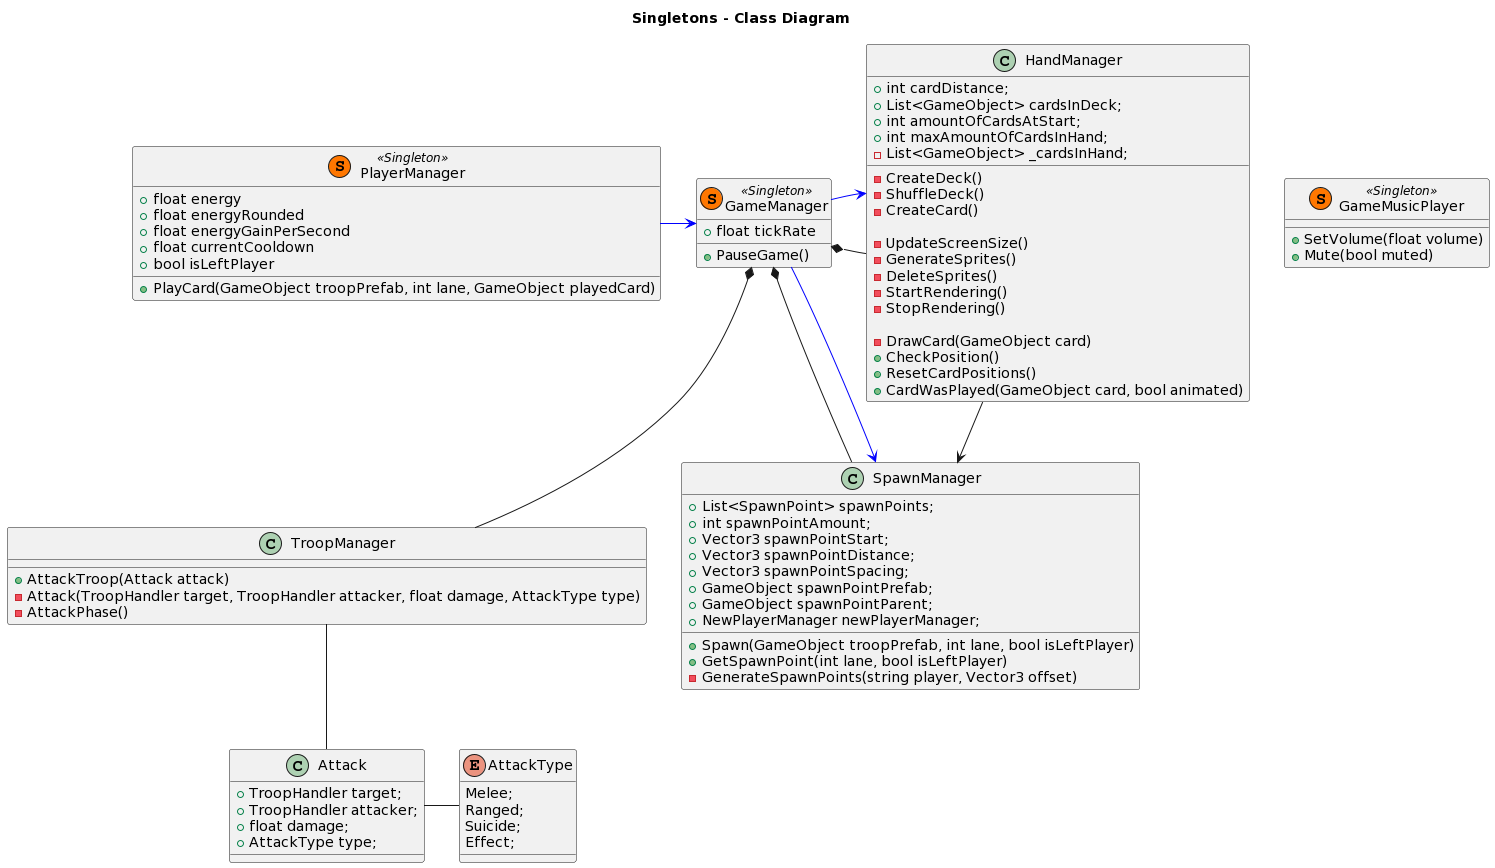
\includegraphics[width=14cm]{resources/Singletons.png} \\
\textit{momentaner Aufbau} \\
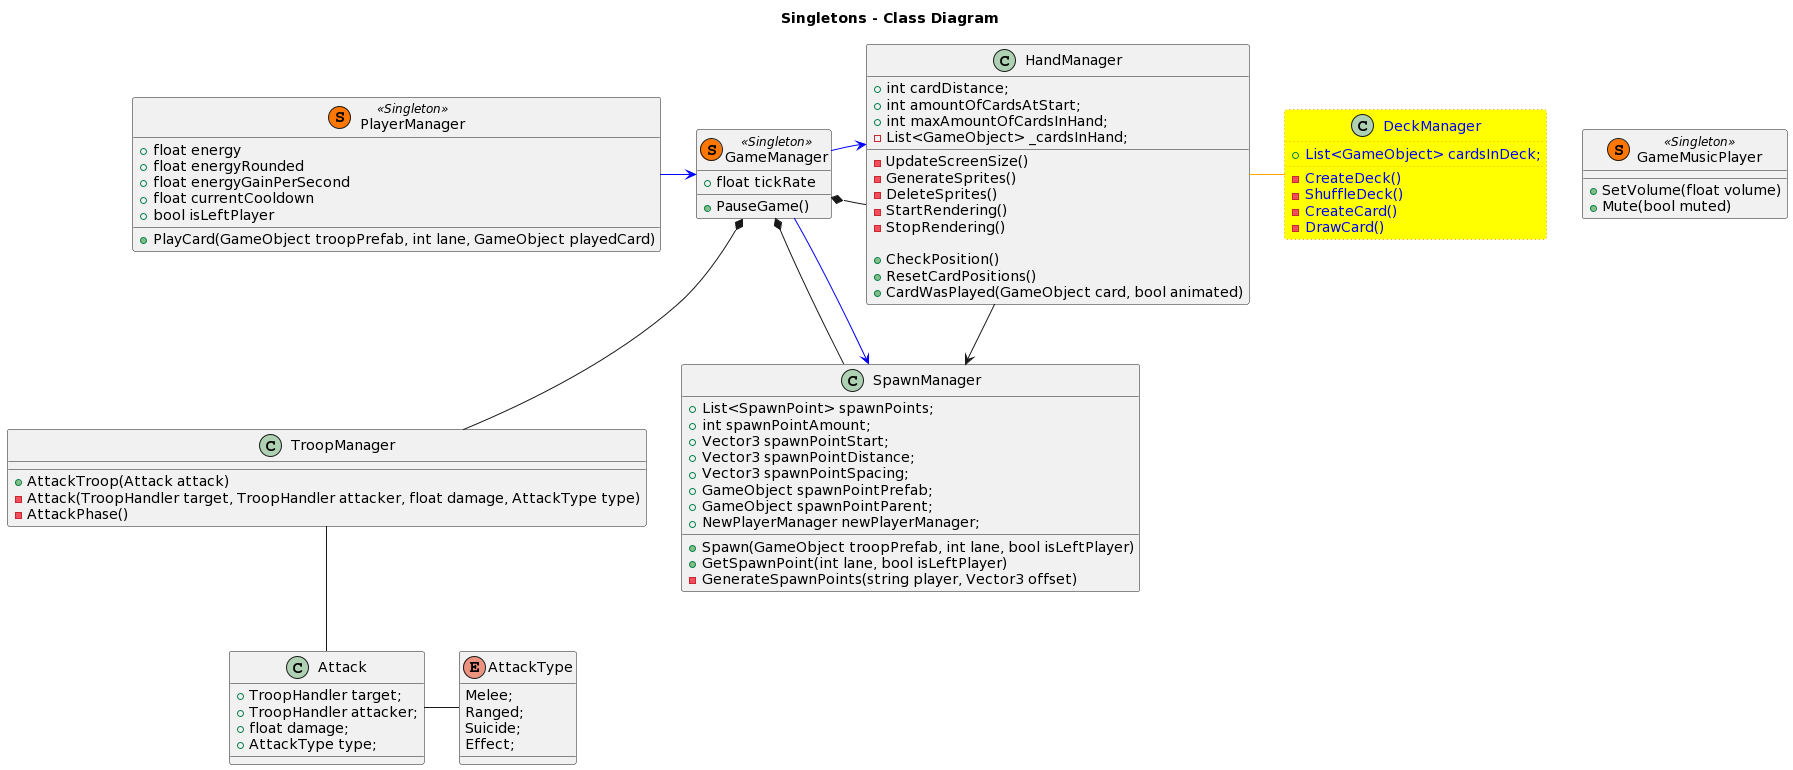
\includegraphics[width=14.5cm]{resources/Singletons 2.png} \\
\textit{zukünftiger Aufbau}

\section{Nahkampftruppe}
Folgend ist die Abfolge unseres Codes zusehen, falls eine Truppe in die Reichweite einer Nahkampftruppe kommt.
Das die Suizidtruppe auf den gleichen Prinzipen basiert, ist sie hier mit der zweiten Abbildung abgebildet. \\
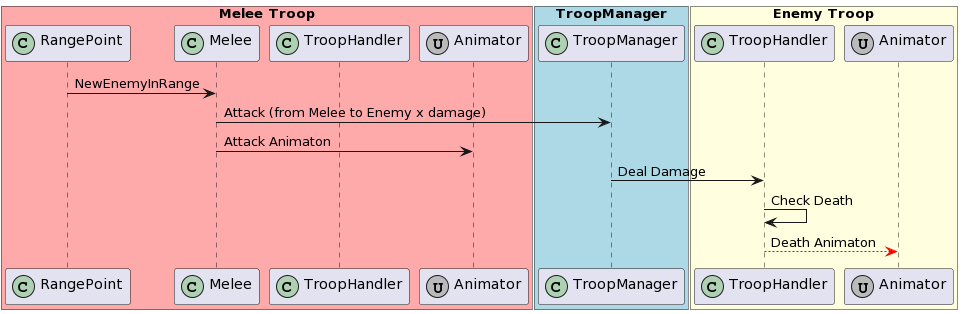
\includegraphics[width=15cm]{resources/MeleeAttacks.png} \\
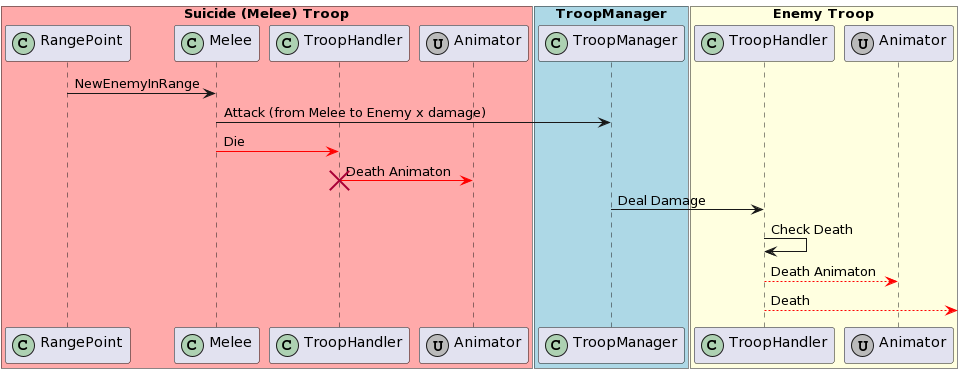
\includegraphics[width=15cm]{resources/SuicideAttacks.png} \\

\section{Fernkampftruppe}
Folgend ist abgebildet wie eine Fernkampftruppe auf einen neuen Gegner reagiert.
Falls der Gegner stirbt und das Projektil nichts trifft, ist auf der zweiten Abbildung abgebildet.
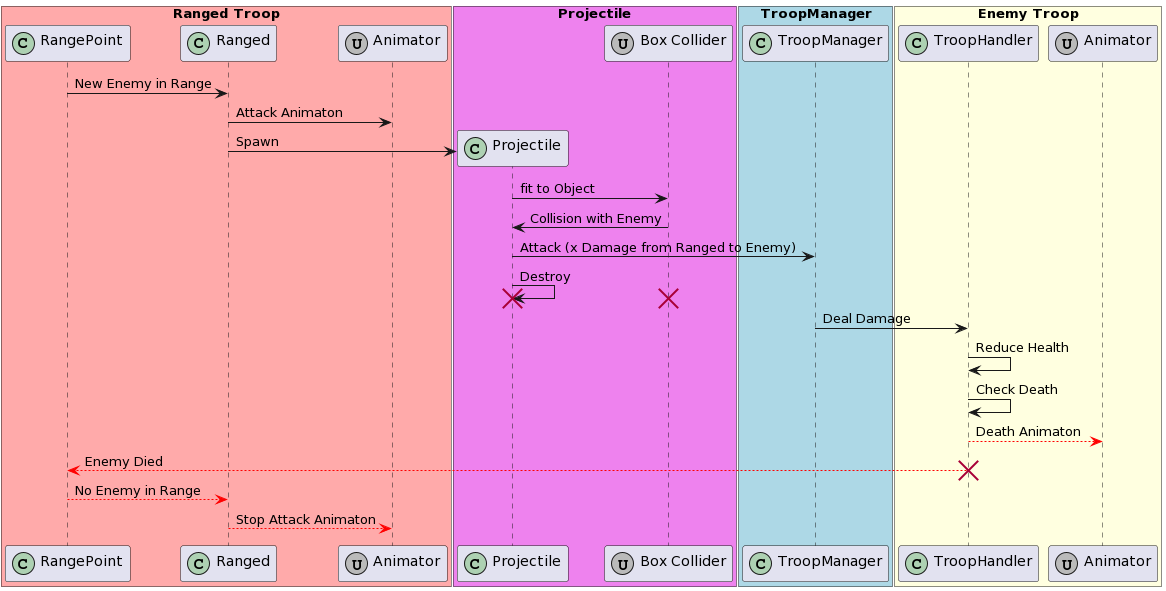
\includegraphics[width=15cm]{resources/RangedAttacks.png} \\
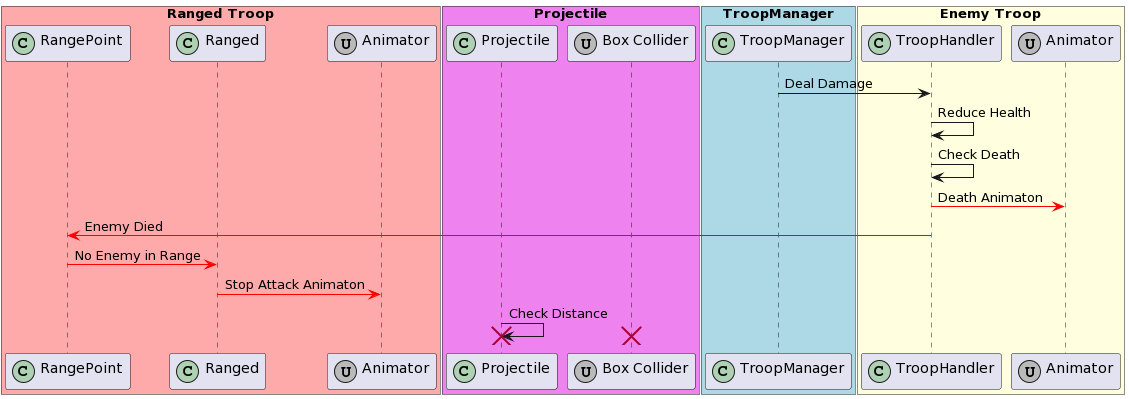
\includegraphics[width=15cm]{resources/Projectile.png}

\section{Gift}
Folgend ist die Sequenz abgebildet, falls eine Giftige Truppe angegriffen wird. \\
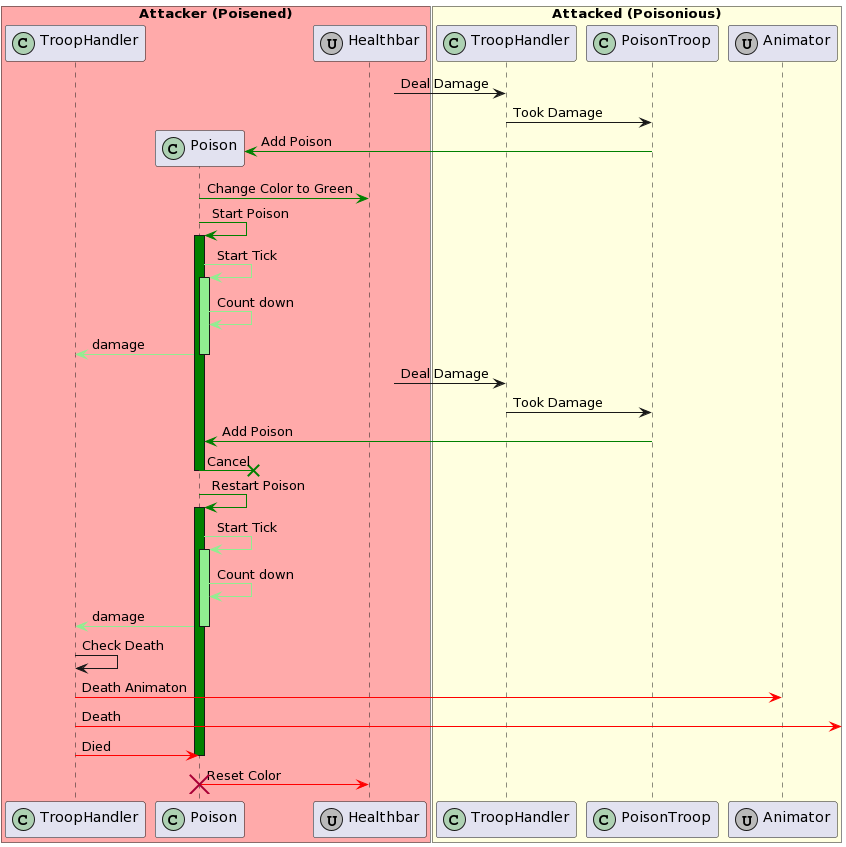
\includegraphics[width=15cm]{resources/Poison.png} \\


\section*{github file system / source / version control}
\url{https://www.youtube.com/watch?v=IQT37uwpcg4}